\section{Cloud und Edge Robotic Architekturen} % (fold)
\label{sec:Cloud und Edge Robotic Architekturen}

Die Nutzung von Cloud und Edge Computing Ressourcen in Kombination mit Robotern öffnet die Möglichkeit für verschiedene Arten von Architekturen. Neben der einfachen Kommunikation zwischen Robotern, ermöglichen Edge und Cloud Server komplexere Systeme die zum Beispiel bei dem effizienteren Auslagern von Ressourcen genutzt werden können. Vor allem Dezentralisierte Architekturen sind diesbezüglich interessant. Roboter können dabei die Speicherung von Daten oder Ausführung von Rechenleistung an einem anderen Knoten in einem System auslagern. In \cite{jawharNetworkingMultiRobotSystems2018} beschreibt Imad Jawhar et al. verschiedene Architekturen die sich im Speziellen auf Multi Roboter Systeme beziehen. Dabei nennt er vier Architekturen:

\begin{enumerate}
  \item Zentralisierte: Hier gibt es einen Zentralen Knoten der alle Clients verwaltet. Problem hierbei ist ganz klar der Single point of failure und die Skalierung.
    \item Hierarchische: Bei dieser Art der Architektur gibt es mehrere übergeordnete Steuerungsknoten. Dieses Konzept kann man näherungsweise mit einer Edge Architektur vergleichen. Der Vorteil von dieser Architektur ist die Skalierung. Beim hinzufügen von Robotern können weitere Instanzen, Beispielweise im Edge, hinzugefügt werden. Nachteil ist die Zuverlässigkeit, da insgesamt mehr Instanzen involviert sind.
      \item Dezentralisiert: Wie eingangs Erwähnt hat man hier keine zentrale Instanz. Dadurch ist das System sehr robust, jedoch auf Kosten der Synchronisation die komplexer ist.
        \item Hybrid: Nach den Autoren des Papers, ist dies in Multi Roboter Systemen die Populärste Alternative. Dabei kombiniert man verschiedene der oben genannten Architekturen um eine gute Balance zwischen der Skalierbarkeit von dezentralisierten und der Zuverlässigkeit von zentraleren Modellen.
\end{enumerate}

Im folgenden werden verschiedene Arten von Netzwerk Teilnehmern und deren Eigenschaften in einem Cloud und Edge Robotics Netzwerk beschrieben. Darauf aufbauend, werden dann drei Arten von Architekturen für Cloud und Edge Robotics erläutert und jeweils die Anwendung im Transportprotokoll Zenoh erläutert.\\

Die erste Art von von Teilnehmer ist ein einfacher Client. Dieser dient als Endanwender im System. Er kann auf Topics im Netzwerk subscriben oder selber Daten publishen. Im Gegensatz zu den weiteren Teilnehmern, kann ein Client kein Routing vornehmen. Im Kontext dieser Arbeit, ist ein Roboter oder Microcontroller ein Beispiel für ein Client. Dieser sendet Umgebungsdaten und Sensordaten aus und bekommt Steuerungsbefehle aus dem Netzwerk. In Zenoh können Clients auf verschiedenster Weise Implementiert werden. Dafür bietet Zenoh verschiedene Client Bibliotheken an. Beispielsweise für Rust, Python oder C. Speziell ist ebenfalls die Pico Client Bibliothek, die es ermöglicht sehr leistungsschwache Geräte zu unterstützen.\\
Im Gegensatz zum Client steht der Router. Dieser ist ausschließlich für die Weiterleitung von Daten und Befehlen zuständig und hat keine Rolle als Anwendung. Zenoh bietet hierfür ein Kommandozeilentool(\code{zenohd}) an welches unter anderem für verschiedene Plattformen als einfache Binäre Datei zur Verfügung steht. Der Zenoh Router lässt sich dabei leicht mittels Kommandozeilenparameter oder einer Konfigurationsdatei für den jeweiligen Use Case anpassen. Ein Beispiel hierfür sind die Anbindungen an Datenbanken oder andere Speichermöglichkeiten. Damit ist es möglich, neben den bekannten Publish/Subscribe Funktionalitäten, Daten per \code{PUT} Query abzuspeichern.\\
Schlussendlich gibt es noch sogenannte Peers. Diese stellen eine Mischung aus Client und Router dar. Das heißt, dass sie sowohl Anwendungs als auch Routing Fähigkeiten haben. Bekannt sind Peers aus dem Peer-to-Peer Netzwerkmodell. In Zenoh lässt sich ein Peer aus der Nutzung von einer Client Bibliothek und dem Zenoh Router nutzen. Beispielsweise könnte ein leistungsstarker Cloud Server Nachrichten sowohl Routen als auch die im Zenoh Speicher abgelegten Daten direkt zu Weiterverarbeitung in einem Machine Learning Model nutzen.\\

Bei den Netzwerk Architekturen gibt es im Cloud und Edge Bereich auch drei große Kategorien. Peer-to-Peer Netze, Router und Broker basierte Architekturen.\\
Die erste Art von Architekturen sind Peer-to-Peer Netze \cite{schollmeierDefinitionPeertoPeerNetworking2001}. Diese nutzen Peers um miteinander zu kommunizieren. Im Cloud und Edge Computing Bereich, könnte man diese als Server darstellen die jeweils eine Aufgabe ausführen und miteinander kommunizieren. Hier wäre eine Kombination zwischen Rechnern an der Edge und in der Cloud vorstellbar. Die Anwendung könnte hier Beispielweise die Auswertung der Daten im Edge Server und die weiterverarbeitung in einer Leistungsstärkeren Cloud Instanz sein. Spezialfälle von Peer-to-Peer Netzwerke sind Mesh \cite{cilfoneWirelessMeshNetworking2019} und Clique \cite{enwiki:1096684789} Netzwerke. Erstere charakterisieren sich dadurch, dass sie zusammenhängend sind. Man kann also von jedem Knoten, jeden anderen Knoten erreichen. Falls keine direkte Verbindung existiert, kann dafür auch ein Umweg über einen weiteren Knoten genommen werden. Bei Clique Peer-to-Peer Netzwerke, hat jeder Knoten eine Verbindung zu jedem anderen Knoten. Dies kann man dann ausnutzen und die direkten Verbindungen zwischen den Peers ausnutzen. Zenoh unterstützt dank dem dynamischen discovery Mechanismus automatisch alle Arten von Peer-to-Peer Typologie.\\
Router basierte Architekturen sind die zweite Art von Architekturen. Hier stehen Router im Vordergrund um Nachrichten zwischen verschiedenen Clients und Peers auszutauschen. Wie im Use Case \ref{sub:Steuerung über WAN (Internet)} zu sehen, eignet sich diese Art der Architektur gut für die Skalierung über weit entfernte Netze. Beispielsweise über das Internet. Nachrichten können auch über mehrere Router weitergeleitet werden. Dies ist in Abbildung \ref{fig:Cloud und Edge Robotics Architekturen} der Fall. Hier ist ein Client mit jeweils einem eigenen Router verbunden. Um Nachrichten von einem Client zum anderen austauschen zu können, müssen diese über beide Router geleitet werden.\\
Das letzte relevante Architektur Muster im Cloud und Edge Robotics Bereich ist der Broker basierte Ansatz. Dieser ist aus Message Queues wie RabbitMQ \cite{AMQP091Model} bekannt und ähnelt der Router basierten Architektur. In diesem Fall sind aber alle Clients mit dem gleichen Router verbunden. Das heißt, dass alle Clients diesen nutzen müssen um Nachrichten auszutauschen. Im Falle einer Roboterflotte kann ein zentraler Broker eine gute Idee sein. Nachrichten können dann Zentral weitergeleitet werden und Konflikte sind einfacher vorzubeugen.\\

\begin{figure}
  \begin{center}
    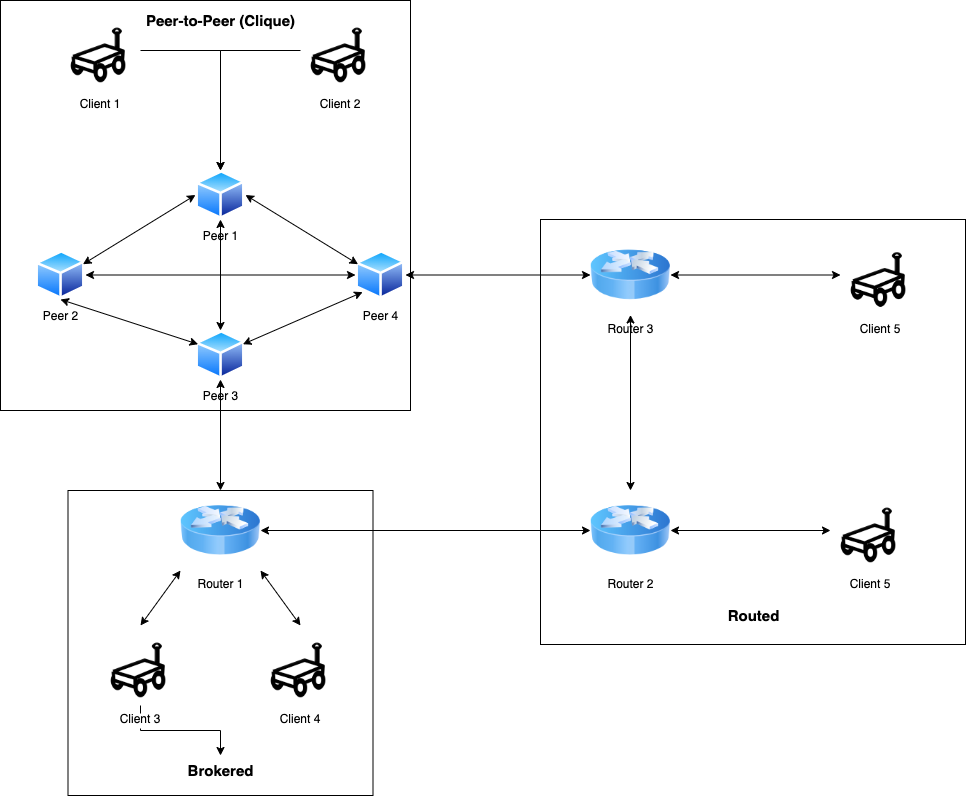
\includegraphics[width=0.8\textwidth]{figures/topologies.drawio.png}
  \end{center}
  \caption{Cloud und Edge Robotics Architekturen}
  \label{fig:Cloud und Edge Robotics Architekturen}
\end{figure}

In \ref{fig:Cloud und Edge Robotics Architekturen} sind die die drei zuvor beschriebenen Architekturen mit den jeweiligen Teilnehmern dargestellt. Oben Links ist die Peer-to-Peer Architektur mit dem Sonderfall einer Clique dargestellt. Diese beinhaltet ebenfalls einen Broker basierten Teil, da \textit{Client 1} und \textit{Client 2} jeweils über \textit{Peer 1} gehen müssen um miteinander zu kommunizieren. Rechts davon befindet sich eine Router basierte Architektur, wie auch im oberen Abschnitt beschrieben. Beide \textit{Clients 5/6} müssen jeweils über Ihre eigenen Router gehen um mit anderen Teilnehmern zu kommunizieren. Schlussendlich ist im unteren Bereich wieder eine Broker basierte Architektur abgebildet wie sie zuvor schon beschrieben wurde.

% section Cloud und Edge Robotic Architekturen (end)
